\begin{flushright} {\tiny {\color{gray} compgeo.tex}} \end{flushright}

\section{Convection in a box *}

This exercise builds on your existing 2D advection-diffusion code. 
Scale up the benchmark described in Section~\ref{sec:ldc_anal} so that 
it runs in a 1000x1000 km domain with Earth-like parameters and velocities
(the maximum velocity is denoted by $\upnu_{conv}$ and will be varied).
Start with an initial zero temperature field and Earth-like boundary conditions 
on the top and bottom, e.g. $T=20$ at the top and $T=1000$ at the bottom. 
Set $k=3$, $C_p=1250$ and $\rho=3000$.

Run the code until steady state is reached. Implement an algorithm which computes the average 
temperature 
\[
<T> = \frac{1}{L_xL_y} \iint T(x,y) dx dy
\]
in the domain and plot it as a function of time.
Also compute the root mean square velocity in the domain:
\[
\upnu_{rms} = \sqrt{   \frac{1}{L_xL_y} \iint (u^2+v^2) dx dy  }
\]
Plot the steady state $<T>$ and $\upnu_{rms} $ as a function of the resolution $h$. 
Plot the temperature on the $x=L_x/2$ line for different values 
of $\upnu_{conv}$.
When possible, make a link with the Mantle Dynamics practical. 

Bonus: Compute and plot the heat flux $\vec{q}=-\vec\nabla T$ in the center of the elements.

%-------------------------------------------
\section{Corner flow subduction *}

\begin{itemize}
\item In this experiment the velocity is prescribed in geometrically simple subducting and overriding plates,
while the velocity in the mantle is computed by means of an analytical solution coined 'corner flow velocity'.
Details are to be found in G.K. Batchelor, {\it An introduction to fluid dynamics}. Cambridge University Press, 1967.
\item Write a function which prescribes the velocity in a lithospheric sized domain.
\item Use this velocity to drive the system in time (choose the appropriate values for the coefficients in the heat 
transport equation)
\item prescribe a constant temperature value at the top, and fix the temperature on both sides, but only in the 
plates (along lengths $l_1$ and $l_2$. Choose an appropriate plate temperature model.
\item Run the model over millions of years with different velocities.
\item Measure the depth of the isotherm $800^\circ$ as a function of time (bonus). 
\item Is steady state ever reached ?
\end{itemize}

If all goes well, you should be able to recover similar results:

\begin{center}
a)\includegraphics[width=6cm]{images/compgeo/corner1}
\hspace{1cm}
b)\includegraphics[width=7cm]{images/compgeo/corner2}\\
{\captionfont 3D setup with prescribed velocity. b) example of temperature field evolution}
\end{center}

{\color{red} what are l1, l2 ? rephrase !}

%-------------------------------------------
\section{From 2D to 3D **}

Rewrite your 2D FEM advection-diffusion code so that it now runs on a cube. 
You will need to create a new connectivity array, compute new elemental matrices, etc ...
Center the cube on the origin of the axis system.

Compute the steady-state solution of a problem without heat advection. The domain is a unit cube,
$k=\rho=C_p=1$. A temperature $T_{max}=1$ is prescribed at the bottom and $T_{min}=0$ at the top. 

Same problem when these boundary conditions are now prescribed on the faces.

Prescribe an temperature field such that it is 1 everywhere in the domain but 
2 inside a sphere of radius 0.1 centered at $(0.66,0.66,0.66)$.
This time no diffusion takes place but we wish to advect the field using the velocity
$\vec\upnu=(y,x,0)$. What is the highest resolution that is achievable on your computer?


%-------------------------------------------
\section{Triangular linear elements */**}

Redo the 2D advection-diffusion exercises with triangular elements.
You will need to make a new icon array, and recompute the mass matrix 
and other matrices. The triangular elements are constructed by splitting 
square elements along the diagonal.
See Section~\ref{ss:p1} for the basis functions and their derivatives.
See Appendix~\ref{ss:tle} for the calculations of the matrices.  

%------------------------------------
\section{Triangular linear elements ***}

Same exercise as above, with an additional task: run the benchmark
presented in Section~\ref{sec:hfcyl}.
For this you will need to generate a mesh 
such that nodes are placed on the perimeter of the cylinder and there is 
no node inside the cylinder:

\includegraphics[width=8cm]{images/compgeo/hole}

You can build it 
by hand, or you can use an external mesher library (see Delaunay triangulation inside scipy).
Vary the heat conduction coefficient to show the effect of diffusion on the obtained
steady state temperature field.  



%---------------------------------------
\section{Diffusion of topography ****}

In a 2D plane assign each node an initial topography $h(x,y,t=0)$ given by 
\[
h(x,y,t=0)= h_0 \sin(\pi x/L_x) + \xi(x,y) \delta h
\]
where $L_x$ and $L_y$ are the dimensions of the domain, $h_0$ is the 
height of the orogen, $xi(x,y)$ is a random perturbation in $[-1,1]$
and $\delta h$ is the amplitude of the perturbation.

We wish to 'erode' the topography by means of a (nonlinear) diffusion law
as in section 2.1.1 of Burov \& Cloetingh \cite{bucl97}.

\begin{enumerate}
\item What are the physical parameters needed to carry out this experiment? 
What are the appropriate boundary conditions? 
What is the steady state? What are the relevant time scales? How should we choose the time step?
\item Write a code which solves the linear diffusion equation until steady state is reached.
Explore the effect of $\delta h$. Compute the slope $\vec\nabla h$ inside each element and plot 
its time evolution. 
\item Implement the nonlinear diffusion law and run the model once again. 
\item If a source term is added to the diffusion equation it is in fact a vertical velocity
($\partial h/\partial t$ has the dimensions of a velocity). Add a source term which generates 
uplift in a symmetric and asymmetric manner.  
\end{enumerate}

\Literature  \cite{thsh14} \cite{ster20}, also check Appendix H. 

%-----------------------------------------------
\section{An example of a hand-built triangular mesh}

We start from a 8x5 domain which is tesselated as follows:

\begin{center}
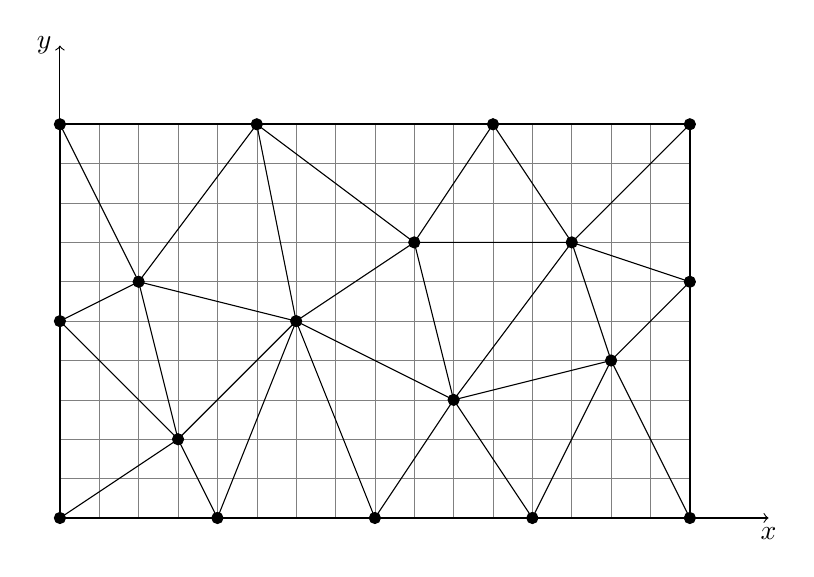
\begin{tikzpicture}
%\draw[fill=gray!8,gray!8](0,0) rectangle (10,7);
\draw[step=0.5cm,gray,very thin] (1,1) grid (9,6); %background grid
\draw[thick] (1,1) -- (9,1) -- (9,6) -- (1,6) -- cycle;  

\draw[thin,->] (1,1) -- (10,1) ; %horizontal axis
\draw[thin,->] (1,1) -- (1,7) ; %horizontal axis
\node[] at (10,0.8){$x$};
\node[] at (0.8,7){$y$};

\draw[] (1,1) -- (2.5,2) -- (4,3.5) -- (5.5,4.5) -- (6.5,6);  %1 6 11 13 14
\draw[] (3,1) -- (4,3.5) -- (6,2.5) -- (7.5,4.5) -- (9,6) ;  %2 11 12 15 16
\draw[] (3,1) -- (2.5,2) -- (1,3.5) -- (2,4) -- (1,6) ;  %2 6 7 8 9
\draw[] (5,1) -- (6,2.5) -- (7,1) -- (8,3) -- (9,4) -- (7.5,4.5) -- (6.5,6) ;  %3 12 4 18 17 15 14
\draw[] (3.5,6) -- (2,4) -- (4,3.5) -- (5,1) ;  %10 8 11 3
\draw[] (2.5,2) -- (2,4) ; %6 8
\draw[] (4,3.5) -- (3.5,6) -- (5.5,4.5) -- (7.5,4.5) ;  %11 10 13 15
\draw[] (9,1) -- (8,3) -- (6,2.5) -- (5.5,4.5) ;  %5 18 12 13
\draw[] (7.5,4.5) -- (8,3) ; %15 18

\draw[black,fill=black] (1,1)     circle (2pt); 
\draw[black,fill=black] (3,1)     circle (2pt); 
\draw[black,fill=black] (5,1)     circle (2pt); 
\draw[black,fill=black] (7,1)     circle (2pt); 
\draw[black,fill=black] (9,1)     circle (2pt); 
\draw[black,fill=black] (2.5,2)   circle (2pt); 
\draw[black,fill=black] (1,3.5)   circle (2pt); 
\draw[black,fill=black] (2,4)     circle (2pt); 
\draw[black,fill=black] (1,6)     circle (2pt); 
\draw[black,fill=black] (3.5,6)   circle (2pt); 
\draw[black,fill=black] (4,3.5)   circle (2pt); 
\draw[black,fill=black] (6,2.5)   circle (2pt); 
\draw[black,fill=black] (5.5,4.5) circle (2pt); 
\draw[black,fill=black] (6.5,6)   circle (2pt); 
\draw[black,fill=black] (7.5,4.5) circle (2pt); 
\draw[black,fill=black] (9,6)     circle (2pt); 
\draw[black,fill=black] (9,4)     circle (2pt); 
\draw[black,fill=black] (8,3)     circle (2pt); 

\end{tikzpicture}\\
\end{center}
         
We can first label the nodes:

\begin{center}
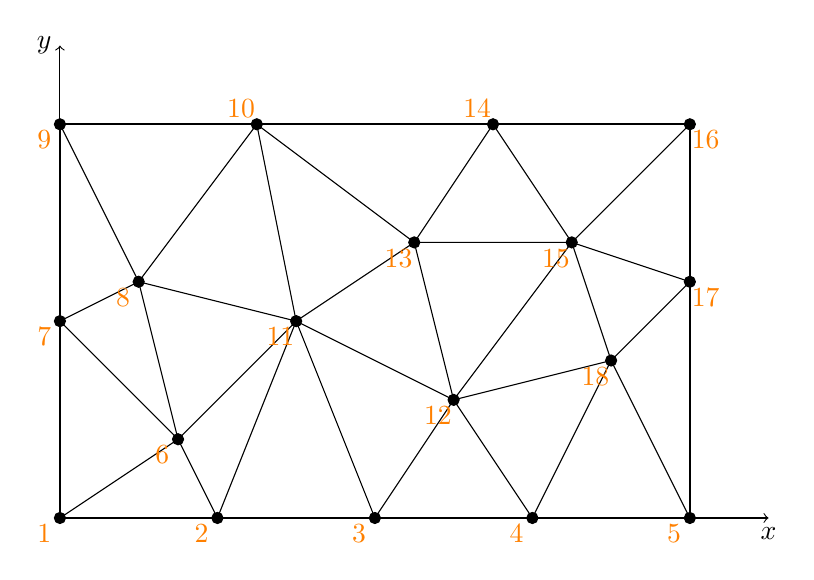
\begin{tikzpicture}
%\draw[fill=gray!5,gray!5](0,0) rectangle (10,7);
%\draw[step=0.5cm,gray,very thin] (1,1) grid (9,6); %background grid
\draw[thick] (1,1) -- (9,1) -- (9,6) -- (1,6) -- cycle;  

\draw[thin,->] (1,1) -- (10,1) ; %horizontal axis
\draw[thin,->] (1,1) -- (1,7) ; %horizontal axis
\node[] at (10,0.8){$x$};
\node[] at (0.8,7){$y$};


\draw[] (1,1) -- (2.5,2) -- (4,3.5) -- (5.5,4.5) -- (6.5,6);  %1 6 11 13 14
\draw[] (3,1) -- (4,3.5) -- (6,2.5) -- (7.5,4.5) -- (9,6) ;  %2 11 12 15 16
\draw[] (3,1) -- (2.5,2) -- (1,3.5) -- (2,4) -- (1,6) ;  %2 6 7 8 9
\draw[] (5,1) -- (6,2.5) -- (7,1) -- (8,3) -- (9,4) -- (7.5,4.5) -- (6.5,6) ;  %3 12 4 18 17 15 14
\draw[] (3.5,6) -- (2,4) -- (4,3.5) -- (5,1) ;  %10 8 11 3
\draw[] (2.5,2) -- (2,4) ; %6 8
\draw[] (4,3.5) -- (3.5,6) -- (5.5,4.5) -- (7.5,4.5) ;  %11 10 13 15
\draw[] (9,1) -- (8,3) -- (6,2.5) -- (5.5,4.5) ;  %5 18 12 13
\draw[] (7.5,4.5) -- (8,3) ; %15 18

\draw[black,fill=black] (1,1)     circle (2pt); \node[] at (0.8,0.8){\color{orange} 1}; %1
\draw[black,fill=black] (3,1)     circle (2pt); \node[] at (2.8,0.8){\color{orange} 2}; %2
\draw[black,fill=black] (5,1)     circle (2pt); \node[] at (4.8,0.8){\color{orange} 3}; %3
\draw[black,fill=black] (7,1)     circle (2pt); \node[] at (6.8,0.8){\color{orange} 4}; %4
\draw[black,fill=black] (9,1)     circle (2pt); \node[] at (8.8,0.8){\color{orange} 5}; %5
\draw[black,fill=black] (2.5,2)   circle (2pt); \node[] at (2.3,1.8){\color{orange} 6}; %6
\draw[black,fill=black] (1,3.5)   circle (2pt); \node[] at (0.8,3.3){\color{orange} 7}; %7
\draw[black,fill=black] (2,4)     circle (2pt); \node[] at (1.8,3.8){\color{orange} 8}; %8
\draw[black,fill=black] (1,6)     circle (2pt); \node[] at (0.8,5.8){\color{orange} 9}; %9
\draw[black,fill=black] (3.5,6)   circle (2pt); \node[] at (3.3,6.2){\color{orange} 10};%10
\draw[black,fill=black] (4,3.5)   circle (2pt); \node[] at (3.8,3.3){\color{orange} 11};%11
\draw[black,fill=black] (6,2.5)   circle (2pt); \node[] at (5.8,2.3){\color{orange} 12};%12
\draw[black,fill=black] (5.5,4.5) circle (2pt); \node[] at (5.3,4.3){\color{orange} 13};%13
\draw[black,fill=black] (6.5,6)   circle (2pt); \node[] at (6.3,6.2){\color{orange} 14};%14
\draw[black,fill=black] (7.5,4.5) circle (2pt); \node[] at (7.3,4.3){\color{orange} 15};%15
\draw[black,fill=black] (9,6)     circle (2pt); \node[] at (9.2,5.8){\color{orange} 16};%16
\draw[black,fill=black] (9,4)     circle (2pt); \node[] at (9.2,3.8){\color{orange} 17};%17
\draw[black,fill=black] (8,3)     circle (2pt); \node[] at (7.8,2.8){\color{orange} 18};%18
\end{tikzpicture}\\
\end{center}

and then label the elements:

\begin{center}
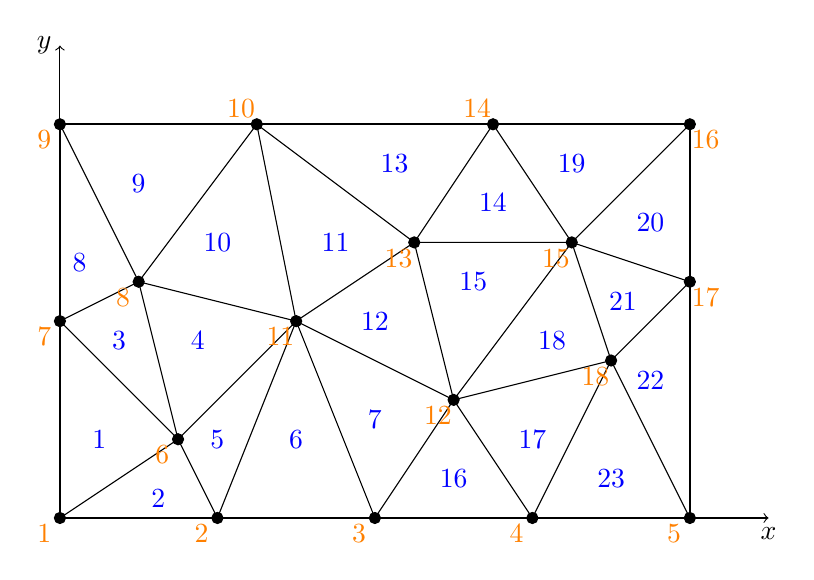
\begin{tikzpicture}
%\draw[fill=gray!5,gray!5](0,0) rectangle (10,7);
%\draw[step=0.5cm,gray,very thin] (1,1) grid (9,6); %background grid
\draw[thick] (1,1) -- (9,1) -- (9,6) -- (1,6) -- cycle;  

\draw[thin,->] (1,1) -- (10,1) ; %horizontal axis
\draw[thin,->] (1,1) -- (1,7) ; %horizontal axis
\node[] at (10,0.8){$x$};
\node[] at (0.8,7){$y$};


\draw[] (1,1) -- (2.5,2) -- (4,3.5) -- (5.5,4.5) -- (6.5,6);  %1 6 11 13 14
\draw[] (3,1) -- (4,3.5) -- (6,2.5) -- (7.5,4.5) -- (9,6) ;  %2 11 12 15 16
\draw[] (3,1) -- (2.5,2) -- (1,3.5) -- (2,4) -- (1,6) ;  %2 6 7 8 9
\draw[] (5,1) -- (6,2.5) -- (7,1) -- (8,3) -- (9,4) -- (7.5,4.5) -- (6.5,6) ;  %3 12 4 18 17 15 14
\draw[] (3.5,6) -- (2,4) -- (4,3.5) -- (5,1) ;  %10 8 11 3
\draw[] (2.5,2) -- (2,4) ; %6 8
\draw[] (4,3.5) -- (3.5,6) -- (5.5,4.5) -- (7.5,4.5) ;  %11 10 13 15
\draw[] (9,1) -- (8,3) -- (6,2.5) -- (5.5,4.5) ;  %5 18 12 13
\draw[] (7.5,4.5) -- (8,3) ; %15 18

\draw[black,fill=black] (1,1)     circle (2pt); \node[] at (0.8,0.8){\color{orange} 1}; %1
\draw[black,fill=black] (3,1)     circle (2pt); \node[] at (2.8,0.8){\color{orange} 2}; %2
\draw[black,fill=black] (5,1)     circle (2pt); \node[] at (4.8,0.8){\color{orange} 3}; %3
\draw[black,fill=black] (7,1)     circle (2pt); \node[] at (6.8,0.8){\color{orange} 4}; %4
\draw[black,fill=black] (9,1)     circle (2pt); \node[] at (8.8,0.8){\color{orange} 5}; %5
\draw[black,fill=black] (2.5,2)   circle (2pt); \node[] at (2.3,1.8){\color{orange} 6}; %6
\draw[black,fill=black] (1,3.5)   circle (2pt); \node[] at (0.8,3.3){\color{orange} 7}; %7
\draw[black,fill=black] (2,4)     circle (2pt); \node[] at (1.8,3.8){\color{orange} 8}; %8
\draw[black,fill=black] (1,6)     circle (2pt); \node[] at (0.8,5.8){\color{orange} 9}; %9
\draw[black,fill=black] (3.5,6)   circle (2pt); \node[] at (3.3,6.2){\color{orange} 10};%10
\draw[black,fill=black] (4,3.5)   circle (2pt); \node[] at (3.8,3.3){\color{orange} 11};%11
\draw[black,fill=black] (6,2.5)   circle (2pt); \node[] at (5.8,2.3){\color{orange} 12};%12
\draw[black,fill=black] (5.5,4.5) circle (2pt); \node[] at (5.3,4.3){\color{orange} 13};%13
\draw[black,fill=black] (6.5,6)   circle (2pt); \node[] at (6.3,6.2){\color{orange} 14};%14
\draw[black,fill=black] (7.5,4.5) circle (2pt); \node[] at (7.3,4.3){\color{orange} 15};%15
\draw[black,fill=black] (9,6)     circle (2pt); \node[] at (9.2,5.8){\color{orange} 16};%16
\draw[black,fill=black] (9,4)     circle (2pt); \node[] at (9.2,3.8){\color{orange} 17};%17
\draw[black,fill=black] (8,3)     circle (2pt); \node[] at (7.8,2.8){\color{orange} 18};%18


\node[] at (1.5,2) {\color{blue}1};
\node[] at (2.25,1.25) {\color{blue}2};
\node[] at (1.75,3.25) {\color{blue}3};
\node[] at (2.75,3.25) {\color{blue}4};
\node[] at (3,2) {\color{blue}5};
\node[] at (4,2) {\color{blue}6};
\node[] at (5,2.25) {\color{blue}7};
\node[] at (1.25,4.25) {\color{blue}8};
\node[] at (2,5.25) {\color{blue}9};
\node[] at (3,4.5) {\color{blue}10};
\node[] at (4.5,4.5) {\color{blue}11};
\node[] at (5,3.5) {\color{blue}12};
\node[] at (5.25,5.5) {\color{blue}13};
\node[] at (6.5,5) {\color{blue}14};
\node[] at (6.25,4) {\color{blue}15};
\node[] at (6,1.5) {\color{blue}16};
\node[] at (7,2) {\color{blue}17};
\node[] at (7.25,3.25) {\color{blue}18};
\node[] at (7.5,5.5) {\color{blue}19};
\node[] at (8.5,4.75) {\color{blue}20};
\node[] at (8.15,3.75) {\color{blue}21};
\node[] at (8.5,2.75) {\color{blue}22};
\node[] at (8,1.5) {\color{blue}23};


\end{tikzpicture}\\
\end{center}

We can finally build the connectivity array by hand:

\noindent
icon(1,{\color{blue}1})={\color{orange}1}\\
icon(2,{\color{blue}1})={\color{orange}6}\\
icon(3,{\color{blue}1})={\color{orange}7}\\
icon(1,{\color{blue}2})={\color{orange}1}\\
icon(2,{\color{blue}2})={\color{orange}2}\\
icon(3,{\color{blue}2})={\color{orange}6}\\
icon(1,{\color{blue}3})={\color{orange}7}\\
icon(2,{\color{blue}3})={\color{orange}6}\\
icon(3,{\color{blue}3})={\color{orange}8}\\
...\\
icon(1,{\color{blue}12})={\color{orange}11}\\
icon(2,{\color{blue}12})={\color{orange}12}\\
icon(3,{\color{blue}12})={\color{orange}13}\\
...\\
icon(1,{\color{blue}19})={\color{orange}14}\\
icon(2,{\color{blue}19})={\color{orange}15}\\
icon(3,{\color{blue}19})={\color{orange}16}\\


The labelling of nodes and elements above is done by a human so it starts at 1. When 
implementing this in python, you know what to do ...


%-----------------------------------------------
\section{How to visualise data on a triangular mesh with Paraview}

If arrays {\tt x,y} contain the coordinates of the nodes, your connectivity array is called {\tt icon},
and your mesh consistes of {\tt nel} elements and comprises {\tt nnp} nodes, you can use the following code
to generate a vtu file to be opened with Paraview. You also need a temperature array {\tt T}.

\begin{center}
Code at \url{https://raw.githubusercontent.com/cedrict/fieldstone/master/images/compgeo/mesh_visu.py}
\end{center}

\lstinputlisting[language=python]{images/compgeo/mesh_visu.py}


%==============================================================================
\section{Writing a report as homework \label{app:grading}} 

\begin{itemize}
\item 
The document should contain your full name and student number on the first page. 
\item 
The file should be a pdf which name contains your family name
\item 
Layout: is the document visually pleasing? Is it well structured? 
\item Is there a complete bibliography (when applicable)?
\item Does the structure follows this: Introduction - Methods - Results - Discussion - Conclusion - Appendix ?
\item 
Figures: Are they properly numbered? captioned? all figures must be referenced in the text. 
Are they of good enough quality (no visible pixels)? are they readable? are all axis labelled?
\item 
Text: Overall quality of the language. Are there still typos? Do all sentence make sense?
\item if you wish to show lines of code, use verbatim or lstlisting\footnote{\url{https://en.wikibooks.org/wiki/LaTeX/Source_Code_Listings}} 
\item 
Discussion: are the results properly discussed, analyzed? are potential problems, errors, limitations discussed?
\item 
Conclusion: Are the findings/results summarized and generalized?
\end{itemize}

\begin{center}
\begin{tabular}{cc}
\hline
No & Yes \\
\hline
\hline
$6.67*10^{-11}$ & $6.67 \times 10^{-11}$ \\
$kg/m^3$ &  kg/m$^{3}$ or kg.m$^{-3}$\\
1x1 & 1$\times$1\\
$cos$ & $\cos$\\
docx file & pdf file \\
'if you do this'& passive form \\ 
\hline
\end{tabular}
\end{center}




%.....................................
\par\noindent\rule{\textwidth}{0.4pt}
\begin{center}
\includegraphics[width=10cm]{images/grading/grey}\\
No grey background
\end{center}


%.....................................
\par\noindent\rule{\textwidth}{0.4pt}
\begin{center}
\includegraphics[width=10cm]{images/grading/numbers}\\
No lists/arrays with numbers
\end{center}

%.....................................
\par\noindent\rule{\textwidth}{0.4pt}
\begin{center}
\includegraphics[width=10cm]{images/grading/arrows2}\\
Too many arrows\\
\includegraphics[width=9cm]{images/grading/arrows1}\\
Poor choice of arrow colour
\end{center}

%.....................................
\par\noindent\rule{\textwidth}{0.4pt}
\begin{center}
\includegraphics[width=8cm]{images/grading/pixels1}
\includegraphics[width=7cm]{images/grading/pixels2}\\
Be careful about how you export your figures. These are unreadable.
\end{center}
 
%.....................................
\par\noindent\rule{\textwidth}{0.4pt}
\begin{center}
\includegraphics[width=8cm]{images/grading/eqs1}\\
Parenthesis too small
\end{center}

%.....................................
\par\noindent\rule{\textwidth}{0.4pt}
\begin{center}
\includegraphics[width=9cm]{images/grading/eqs2}\\
1.6E+10 is not acceptable. Replace by $1.6\cdot 10^{10}$
\end{center}

%.....................................
\par\noindent\rule{\textwidth}{0.4pt}
\begin{center}
\includegraphics[width=7cm]{images/grading/eqs3}\\
Equation number is too close to the equation itself. Use labels, 
do not number equations by hand.
\end{center}

%.....................................
\par\noindent\rule{\textwidth}{0.4pt}
\begin{center}
\includegraphics[width=9cm]{images/grading/eqs4}\\
Formatting of both axis lead to unreadable figure.
\end{center}

%.....................................
\par\noindent\rule{\textwidth}{0.4pt}
\begin{center}
\includegraphics[width=9cm]{images/grading/eqs5}\\
In \LaTeX{}  use \verb!\sum\limits!
\end{center}

%.....................................
\par\noindent\rule{\textwidth}{0.4pt}
\begin{center}
\includegraphics[width=9cm]{images/grading/eqs6}\\
Are so many digits necessary?
\end{center}

%.....................................
\par\noindent\rule{\textwidth}{0.4pt}
\begin{center}
\includegraphics[width=12cm]{images/grading/width}\\
use \verb!\usepackage[cm]{fullpage}! to allow for wider text.
\end{center}

%.....................................
\par\noindent\rule{\textwidth}{0.4pt}
\begin{center}
\includegraphics[width=10cm]{images/grading/figs1}\\
This figure style is to be avoided. Simply use dots and/or lines.
\end{center}

%.....................................
\par\noindent\rule{\textwidth}{0.4pt}
\begin{center}
\includegraphics[width=8cm]{images/grading/figs2}
\end{center}

%.....................................
\par\noindent\rule{\textwidth}{0.4pt}
\begin{center}
\includegraphics[width=6cm]{images/grading/loglogpb}\\
Here Ra and Nu are plotted in log-log scale, not log(Ra) and log(Nu).
\end{center}

%.....................................
\par\noindent\rule{\textwidth}{0.4pt}
\begin{center}
\includegraphics[width=10cm]{images/grading/dots}\\
The dots at the beginning and end of the lines are not necessary.
\end{center}

%.....................................
\par\noindent\rule{\textwidth}{0.4pt}
\begin{center}
\includegraphics[width=11cm]{images/grading/you}\\
Never {\it never} use 'you'. 
\end{center}

%.....................................
\par\noindent\rule{\textwidth}{0.4pt}
\begin{center}
\includegraphics[width=10cm]{images/grading/cross}\\
Do not use 'X' but $\times$ (\verb|\times|).
\end{center}




\begin{itemize}
\item The report should be in \LaTeX 
\item The document should contain your full name and student number on the first page. 
\item The report file should be a pdf which name contains your family name
\item not more than 25 pages. If more, use appendices wisely.
\item document should be structured in two main parts: FDM and FEM.
\item no equations unless necessary to the discussion (still mention the equation that 
you are solving but refer to an external document/article/book for example).
\item use lstlisting package to include code
\item use {\verb| \usepackage[cm]{fullpage} |} to format your document
\item all codes either in appendix or in zip file (bearing your name).
\item a decent introduction (half page to one page) which links the topic of this course to geosciences.
\item discussion of results (stability, convergence, influence of resolution, remarks of all kinds).
\item if you did not succeed in doing a particular exercise, please explain what you think the problem is, 
how you know it is not working, etc ...
\item think about colormaps, image compression
%\item DEADLINE: July 16th, 2023, 23:59 
\end{itemize}


I will use this table to grade your reports:

\vspace{2cm}


\begin{tabular}{|p{5cm}|p{.35cm}|p{.35cm}|p{.35cm}|p{.35cm}|p{.35cm}|p{.35cm}|p{.35cm}|p{.35cm}|p{.35cm}|p{.35cm}|p{.35cm}|p{.35cm}|p{.35cm}|p{.35cm}|p{.35cm}|}
&&&&&&&&&&&&&&& \\
\hline
title, names, student nb &&&&&&&&&&&&&&& \\\hline
\LaTeX ? &&&&&&&&&&&&&&& \\\hline
document layout &&&&&&&&&&&&&&& \\\hline
equations look &&&&&&&&&&&&&&& \\\hline
equations numbered  &&&&&&&&&&&&&&& \\\hline
use of equations &&&&&&&&&&&&&&& \\\hline
figs: caption &&&&&&&&&&&&&&& \\\hline
figs: pixels? &&&&&&&&&&&&&&& \\\hline
figs: correct? &&&&&&&&&&&&&&& \\\hline
English grammar &&&&&&&&&&&&&&& \\\hline
Typos 
Introduction &&&&&&&&&&&&&&& \\\hline
methods/results &&&&&&&&&&&&&&& \\\hline
Discussion/Conclusion  &&&&&&&&&&&&&&& \\\hline
Extra work? &&&&&&&&&&&&&&& \\\hline
Bibliography &&&&&&&&&&&&&&& \\\hline
code layout &&&&&&&&&&&&&&& \\\hline 
code style &&&&&&&&&&&&&&& \\\hline
code accuracy &&&&&&&&&&&&&&& \\\hline
\end{tabular}





